%%%%%%%%%%%%%%%%%%%%
%
%	Final exam (03) : 2024--04--30 (T)
%
%%%%%%%%%%%%%%%%%%%%



\section{Exercise \ref{sec : e03q1}}
\label{sec : e03q1}

\noindent{}Let $R$ be a commutative ring with a multiplicative identity $1_{R} \neq 0_{R}$, and let $I \subseteq R$.
\begin{enumerate}[label=(\alph*)]
\item\label{itm : e03q1a} Define what it means for $I$ to be (i) an ideal, (ii) a prime ideal, and (iii) a maximal ideal.
\item\label{itm : e03q1b} Let $I$ be an ideal of $R$. Prove that if $I$ is maximal, then $I$ is prime. (\fontHint{Use quotient rings.})
\item\label{itm : e03q1c} Give an example to show that the converse to the statement in part \ref{itm : e03q1b} is false, in general. That is, give an example of a prime ideal that is not maximal.
\item\label{itm : e03q1d} For each $i \in \integersPositive$, let $I_{i}$ be an ideal of $R$ such that $I_{1} \subseteq I_{2} \subseteq \ldots$. Prove that $I = \cup_{i \in \integersPositive} I_{i}$ is an ideal of $R$.
%\item\label{itm : e03q1e} Use the ring (???) to show that the statement in part \ref{itm : e03q1c} is false if we replace each instance of ``ideal'' with (i) ``prime ideal'' or (ii) ``maximal ideal''.
\end{enumerate}

\spaceSolution{0in}{% Begin solution.
Part \ref{itm : e03q1a}: Let $I \subseteq R$. $I$ is an \fontDefWord{ideal} of $R$ if it is a subring of $R$ and closed under multiplication by elements of $R$. This is equivalent to the following three conditions:
\begin{enumerate}[label=(\roman*)]
\item Nonempty: $0_{R} \in I$.
\item Closed under $+$: For all $a_{1}, a_{2} \in I$, $a_{1} + a_{2} \in I$.
\item Strongly closed under $\times$: For all $a \in I$, for all $r \in R$, $r a \in I$.
\end{enumerate}
$I$ is a \fontDefWord{prime ideal} of $R$ if it satisfies the following two conditions:
\begin{enumerate}[label=(\roman*)]
\item $I$ is a proper ideal of $R$ (that is, $I \neq R$).
\item For all $r_{1}, r_{2} \in R$, if $r_{1} r_{2} \in I$, then $r_{1} \in I$ or $r_{2} \in I$.
\end{enumerate}
$I$ is a \fontDefWord{maximal ideal} of $R$ if it satisfies the following two conditions:
\begin{enumerate}[label=(\roman*)]
\item $I$ is a proper ideal of $R$.
\item For all ideals $J$ of $R$, if $I \subseteq J$, then either $J = I$ or $J = R$.
\end{enumerate}

Part \ref{itm : e03q1b}: Let $I \subseteq R$ be an ideal. Recall that $I$ is maximal if and only if $R / I$ is a field, and $I$ is prime if and only if $R / I$ is an integral domain. Also recall that a field is an integral domain. Thus
\begin{align*}
&\text{$I$ maximal}
&
&\Leftrightarrow
&
&\text{$R / I$ a field}
&
&\Rightarrow
&
&\text{$R / I$ an integral domain}
&
&\Leftrightarrow
&
&\text{$I$ prime}
\end{align*}

Part \ref{itm : e03q1c}: Consider the ideal $(0)$ in $\Z$. Because $\Z$ is an integral domain, $(0)$ is a prime ideal. Because $\Z$ is not a field, $(0)$ is not a maximal ideal. We can prove these assertions either by using the quotient $\Z / (0) \isomorphism \Z$ (see our response to part \ref{itm : e03q1b}) or by using the definitions directly on the ideal $(0)$ in $\Z$. For example, in the latter approach, let $a, b \in \Z$ such that $a b \in (0)$. This is equivalent to $a b = 0$. Because $\Z$ is an integral domain, this implies that either $a = 0$, equivalent to $a \in (0)$; or $b = 0$, equivalent to $b \in (0)$. Thus by definition, the ideal $(0)$ is prime. $(0)$ is contained in every ideal $(n)$ of $\Z$, which is nonzero if $n \neq 0$ and proper if $n \neq \pm{}1$. Thus the ideal $(0)$ is not maximal.

As another example, let $R$ be an integral domain that is not a field (for example, $R = \Z$ or $R = K[s]$ for $K$ a field and $s$ an indeteminate), let $t$ be an indeterminate, and consider the ideal $(t)$ in $R[t]$. Then $R[t] / (t) \isomorphism R$ is an integral domain but not a field, so the ideal $(t)$ is prime but not maximal.

Part \ref{itm : e03q1d}: We verify that $\cup_{i \in \integersPositive} I_{i}$ satisfies the three axioms of an ideal that we listed in our response to part \ref{itm : e03q1a}.
\begin{enumerate}
\item Nonempty. By hypothesis, for any (in fact, for all) $i \in \integersPositive$, $I_{i}$ is an ideal of $R$, so $0_{R} \in I_{i}$. Hence $0_{R} \in \cup_{i \in \integersPositive} I_{i}$.
\item Closed under $+$. Let $r_{1}, r_{2} \in \cup_{i \in \integersPositive} I_{i}$. Then there exist indices $i_{1}, i_{2} \in \integersPositive$ such that $r_{1} \in I_{i_{1}}$ and $r_{2} \in I_{i_{2}}$. Without loss of generality, suppose that $i_{1} \leq i_{2}$. By hypothesis, $I_{1} \subseteq I_{2} \subseteq \ldots$, so $I_{i_{1}} \subseteq I_{i_{2}}$, and hence $r_{1}, r_{2} \in I_{i_{2}}$. By hypothesis, $I_{i_{2}}$ is an ideal, so $r_{1} + r_{2} \in I_{i_{2}} \subseteq \cup_{i \in \integersPositive} I_{i}$.
\item Strongly closed under $\times$. Let $a \in \cup_{i \in \integersPositive} I_{i}$, and let $r \in R$. Then there exists some index $i_{0} \in \integersPositive$ such that $a \in I_{i_{0}}$. By hypothesis, $I_{i_{0}}$ is an ideal, so $r a \in I_{i_{0}} \subseteq \cup_{i \in \integersPositive} I_{i}$.
\end{enumerate}}% End solution.



\section{Exercise \ref{sec : e03q2}}
\label{sec : e03q2}

\begin{enumerate}[label=(\alph*)]
\item\label{itm : e03q2a} Define (i) integral domain, (ii) principal ideal domain, and (iii) field.
\item\label{itm : e03q2b} Clearly present the logical implications among the following seven algebraic structures (no proof required):
\begin{quote}
abelian group, euclidean domain (ED), field, integral domain (ID), principal ideal domain (PID), ring, unique factorization domain (UFD)
\end{quote}
\item\label{itm : e03q2c} Let $R$ be a PID, and let $I \subseteq R$ be a prime ideal such that $I \neq (0_{R})$. Prove that $I$ is maximal.
\item\label{itm : e03q2d} Now let $R$ be a commutative ring, and let $t$ be an indeterminate. Prove that the polynomial ring $R[t]$ is a PID if and only if $R$ is a field.
\end{enumerate}

\spaceSolution{0in}{% Begin solution.
Part \ref{itm : e03q2a}: Let $R$ be a ring. $R$ is an \fontDefWord{integral domain} if it is commutative, has a multiplicative identity $1_{R} \neq 0_{R}$, and has no zero divisors (that is, no elements $r_{1}, r_{2} \in R \setminus \{0\}$ such that $r_{1} r_{2} = 0_{R}$). $R$ is a \fontDefWord{field} if it is an integral domain such that every nonzero element is a unit (that is, for each $r \in R \setminus \{0_{R}\}$, there exists an $s \in R$ such that $r s = s r = 1_{R}$). $R$ is a \fontDefWord{principal ideal domain (PID)} if every ideal of $R$ is principal; that is, for each ideal $I \subseteq R$, there exists an $r \in R$ such that $I = (r)$.

Part \ref{itm : e03q2b}: The logical implications among these structures are organized as follows:
\begin{center}
field $\Rightarrow$ ED $\Rightarrow$ PID $\Rightarrow$ UFD $\Rightarrow$ ID $\Rightarrow$ ring $\Rightarrow$ abelian group
\end{center}For the final implication, note that by definition a ring is an abelian group under its addition operation (forget the multiplication operation). Each logical implication is strictly one-way. For example, there are euclidean domains that are not fields (for example, the integers).

Part \ref{itm : e03q2c}: Let $I \subseteq R$ be a nonzero prime ideal, and let $J \subseteq R$ be an ideal such that $I \subseteq J$. We wish to show that $J = I$ or $J = R$. By hypothesis, $R$ is a PID, so there exist $p, m \in R$ such that $I = (p)$ and $J = (m)$. Note that $I \neq (0_{R})$ implies $p, m \neq 0_{R}$. By hypothesis, $p \in I \subseteq J = (m)$, so there exists an $r \in R$ such that
\begin{align}
p
=
r m%
\label{eq : e03q2d}
\end{align}
By hypothesis, $I$ is a prime ideal, so $r m = p \in (p) = I$ implies that (i) $r \in I = (p)$ or (ii) $m \in I$. Case (i) implies that there exists an $s \in R$ such that $r = p s$, so by equation \eqref{eq : e03q2d},
\begin{align*}
p
&=
r m
=
p s m
&
&\Leftrightarrow
&
p (1_{R} - s m)
&=
0_{R}
&
&\Leftrightarrow
&
s m
&=
1_{R}
\end{align*}
where the final equivalence follows from the hypothesis that $R$ is a PID (hence an integral domain) and the earlier observation that $p \neq 0_{R}$. Because $J$ is an ideal, it is strongly closed under multiplication, so $1_{R} = s m \in (m) = J$. Hence $(1_{R}) \subseteq J$, so $J = R$. Case (ii) implies that $J = (m) \subseteq I$, hence $J = I$.

Part \ref{itm : e03q2d}: ($\Leftarrow$) Let $R$ be a field. Then we may define a division algorithm on $R[t]$, which gives $R[t]$ the structure of a euclidean domain. Hence $R[t]$ is a PID. ($\Rightarrow$) Let $R[t]$ be a PID. Then by definition, $R[t]$ is an integral domain, hence the isomorphic image of $R$ in $R[t]$ (namely, the constant polynomials) is an integral domain. Consider the nonzero ideal $(t) \subseteq R[t]$. The quotient $R[t] / (t) \isomorphism R$ is an integral domain, which is equivalent to $(t)$ being a prime ideal. By part \ref{itm : e03q2c}, it follows that the ideal $(t)$ is maximal, and hence $R \isomorphism R[t] / (t)$ is a field.}% End solution.



\section{Exercise \ref{sec : e03q3}}
\label{sec : e03q3}

\noindent{}Let $t$ be an indeterminate. We may give $\Q[t]$ the structure of a ring, a $\Q[t]$-module, or a $\Z$-module. For each map below, state whether it is a ring homomorphism, a $\Q[t]$-module homomorphism, or a $\Z$-module homomorphism. Justify your assertions. \fontHint{A given map may satisfy several or none of these conditions.}
\begin{align*}
\varphi_{1}
:
\Q[t]
&\rightarrow
\Q[t]
&
\varphi_{2}
:
\Q[t]
&\rightarrow
\Q[t]
&
\varphi_{3}
:
\Q[t]
&\rightarrow
\Q[t]
\\
f(t)
&\mapsto
0
&
f(t)
&\mapsto
2 f(t)
&
f(t)
&\mapsto
f(t^{2})
\end{align*}

\spaceSolution{0in}{% Begin solution.
Let $f_{1}, f_{2} \in \Q[t]$. We compute
\begin{align*}
\varphi_{1}(f_{1} + f_{2})
&=
0
=
0 + 0
=
\varphi_{1}(f_{1}) + \varphi_{2}(f_{2})
\\
\varphi_{2}(f_{1} + f_{2})
&=
2 (f_{1} + f_{2})
=
2 f_{1} + 2 f_{2}
=
\varphi_{2}(f_{1}) + \varphi_{2}(f_{2})
\\
\varphi_{3}(f_{1} + f_{2})
&=
(f_{1} + f_{2})(t^{2})
=
f_{1}(t^{2}) + f_{2}(t^{2})
=
\varphi_{3}(f_{1}) + \varphi_{3}(f_{2})
\end{align*}
Thus each map is a homomorphism of abelian groups, which is equivalent to being a $\Z$-module homomorphism.

Next let's check whether each map preserves ring multiplication. We compute
\begin{align*}
\varphi_{1}(f_{1} f_{2})
&=
0
=
0 \cdot 0
=
\varphi_{1}(f_{1}) \varphi_{1}(f_{2})
\\
\varphi_{2}(f_{1} f_{2})
&=
2 (f_{1} f_{2})
\neq
2 f_{1} \cdot 2 f_{2}
=
\varphi_{2}(f_{1}) \varphi_{2}(f_{2})
\\
\varphi_{3}(f_{1} f_{2})
&=
(f_{1} f_{2})(t^{2})
=
f_{1}(t^{2}) f_{2}(t^{2})
=
\varphi_{3}(f_{1}) \varphi_{3}(f_{2})
\end{align*}
where in the second line we have inequality in general (more precisely, we have equality if and only if $f_{1}$ or $f_{2}$ is the zero polynomial). Thus $\varphi_{2}$ is not a ring homomorphism. If we define ring homomorphism to map multiplicative identity to multiplicative identity, then $\varphi_{1}$ is not a ring homomorphism (it maps the constant polynomial $1$ to $0$). If we don't make this restriction in our definition, then $\varphi_{1}$ is a ring homomorphism. For $\varphi_{3}$, our computations for $f_{1} f_{2}$ here and for $f_{1} + f_{2}$ above show that it is a ring homomorphism. Note that $\varphi_{3}(1) = 1$.

Finally, let's check whether each map preserves the scalar multiplication in a $\Q[t]$-module. (Note that $\Q[t]$ is the ring over which the module is defined, so scalars are elements of $\Q[t]$, not just of $\Q$.) We compute
\begin{align*}
\varphi_{1}(f_{1} f_{2})
&=
0
=
f_{1} \cdot 0
=
f_{1} \varphi_{1}(f_{2})
\\
\varphi_{2}(f_{1} f_{2})
&=
2 (f_{1} f_{2})
=
f_{1} 2 f_{2}
=
f_{1} \varphi_{2}(f_{2})
\end{align*}
so $\varphi_{1}$ and $\varphi_{2}$ are $\Q[t]$-module homomorphisms. Taking $f_{1} = f_{2} = t$, we compute
\begin{align*}
\varphi_{3}(t \cdot t)
=
t^{4}
\neq
t \cdot t^{2}
=
t \varphi_{3}(t)
\end{align*}
so $\varphi_{3}$ is not a $\Q[t]$-module homomorphism.

We summarize these results in the table below.
\begin{center}
\begin{tabular}{l l l l}
\hline\hline
Homomorphism of...	&	$\varphi_{1}$	&	$\varphi_{2}$	&	$\varphi_{3}$	\\
\hline
$\Z$-modules			&	Yes					&	Yes					&	Yes					\\
$\Q[t]$-modules		&	Yes					&	Yes					&	No					\\
rings							&	No if we require $1 \mapsto 1$	&	No	&	Yes			\\
								&	Yes otherwise	&							&							\\
\hline
\end{tabular}
\end{center}}% End solution.



\section{Exercise \ref{sec : e03q4}}
\label{sec : e03q4}

\begin{enumerate}[label=(\alph*)]
\item\label{itm : e03q4a} Let $D_{8} = \langle{}r, s \st r^{4}, s^{2}, (r s)^{2}\rangle{}$ be a presentation of the dihedral group of order $8$. For each map below, state whether it defines a valid matrix representation of $D_{8}$. Justify briefly.
\begin{align*}
\rho_{1}
:
D_{8}
&\rightarrow
M_{2}(\Q)
&
\rho_{2}
:
D_{8}
&\rightarrow
M_{2}(\Q)
%&
%\rho_{3}
%:
%D_{8}
%&\rightarrow
%M_{2}(\Q)
\\
r
&\mapsto
\begin{bmatrix}
1	&		\\
	&	1
\end{bmatrix}
&
r
&\mapsto
\begin{bmatrix}
	&	1	\\
-1	&	
\end{bmatrix}
%&
%r
%&\mapsto
%\begin{bmatrix}
%	&	1	\\
%1	&	
%\end{bmatrix}
\\
s
&\mapsto
\begin{bmatrix}
1	&		\\
	&	1
\end{bmatrix}
&
s
&\mapsto
\begin{bmatrix}
	&	1	\\
1	&	
\end{bmatrix}
%&
%s
%&\mapsto
%\begin{bmatrix}
%1	&		\\
%	&	-1
%\end{bmatrix}
\end{align*}
\end{enumerate}
Now let $G$ be a finite group, let $K$ be a field, and let $V$ be a $K$-vector space.
\begin{enumerate}[resume, label=(\alph*)]
%\item\label{itm : e03q4a} Define a (linear) representation of $G$ on $V$.
\item\label{itm : e03q4b} Let $\rho : G \rightarrow \GL(V)$ be a representation of $G$ on $V$. Explain the induced $K G$-module structure on $V$. In particular, specify $(\sum_{g \in G} \alpha_{g} g) \cdot v$, the ring action of the group ring $K G$ on $V$.
\item\label{itm : e03q4c} Define what it means for a module to be (i) decomposable, (ii) reducible, and (iii) completely reducible. (Recall that a representation has one of these properties if the $K G$-module that affords the representation has that property.)
\item\label{itm : e03q4d} Further suppose that $\characteristic K \notDivides \order G$. Let $\rho$ be a matrix representation of $G$ of degree $2$; and let $g_{1}, g_{2} \in G$ such that $\rho(g_{1})$ and $\rho(g_{2})$ do not commute. Prove that $\rho$ is irreducible.
\end{enumerate}

\spaceSolution{0in}{% Begin solution.
Part \ref{itm : e03q4a}: Recall that, by definition, a (linear) representation is a group homomorphism from a group $G$ to the group of invertible linear transformations of a vector space (or matrix representations thereof); and that to check the conditions of a group homomorphism, it suffices to check that the group relations are satisfied. It is straightforward to check that both maps satisfy the required relations on the generators, namely,
\begin{align*}
\rho_{i}(r)^{4}
&=
I
&
\rho_{i}(s)^{2}
&=
I
&
(\rho_{i}(r) \rho_{i}(s))^{2}
&=
I
\end{align*}
where $I$ denotes the $2 \times 2$ identity matrix.

Part \ref{itm : e03q4b}: Let $v \in V$; and note that by definition, any element of $K G$ can be expressed as $\sum_{g \in G} \alpha_{g} g$, where for each $g \in G$, $\alpha_{g} \in K$. Given a representation $\rho : G \rightarrow \GL(V)$, the ring action of $K G$ on $V$ is defined by
\begin{align*}
\left(\sum_{g \in G} \alpha_{g} g\right) \cdot v
=
\sum_{g \in G} \alpha_{g} \rho(g)(v)
\end{align*}
Note that for each $g \in G$, $\rho(g) \in \GL(V)$, so $\rho(g)(v) \in V$, so $\alpha_{g} \rho(g)(v)$ is scalar multiplication of $\alpha_{g} \in K$ on $\rho(g)(v) \in V$ in the $K$-vector space $V$.

Part \ref{itm : e03q4c}: Let $R$ be a ring, and let $M$ be a nonzero $R$-module.
\begin{enumerate}
\item $M$ is \fontDefWord{decomposable} if there exist nonzero submodules $N_{1}, N_{2} \subseteq M$ such that $M = N_{1} \directSum N_{2}$.
\item $M$ is \fontDefWord{reducible} if there exists a nonzero proper submodule $N \subseteq M$.
\item $M$ is \fontDefWord{completely reducible} if there exist irreducible submodules $N_{i} \subseteq M$ such that $M = \oplus_{i} N_{i}$
\end{enumerate}
Note that, in thje setting of matrix representations $\varphi$, these conditions translate as% (!!!) Clarify
\begin{itemize}
\item decomposable $\Leftrightarrow$ nontrivially block-diagonal
\item reducible $\Leftrightarrow$ nontrivally block-upper-triangular
\end{itemize}

Part \ref{itm : e03q4d}: Suppose for the sake of contradiction that $\rho$ is reducible. Then by definition, there exists a nonzero proper $K G$-submodule $N_{1} \subseteq V$, where $V$ is the $K$-vector space underlying the representation $\rho$. (By hypothesis, $\dim_{K} V = 2$.) This is equivalent to $N_{1}$ being a nonzero proper subspace of $V$ that is $G$-invariant. Because $N_{1}$ is nonzero and proper, it follows that $\dim_{K} N_{1} = 1$. By Maschke's theorem, there exists a submodule $N_{2} \subseteq V$ such that $V = N_{1} \directSum N_{2}$. For $i \in \{1, 2\}$, let $v_{i} \in N_{i}$ be a nonzero vector; then $v_{1}, v_{2}$ is a basis of $V$. With respect to this basis (that is, performing a change of basis on the given matrix), the matrix representation of any $g \in G$ is diagonal. In particular, this is true for $g_{1}$ and $g_{2}$. Because $K$ is a field (hence commutative), it follows that $\rho(g_{1})$ and $\rho(g_{2})$ commute, a contradiction.}% End solution.



\section{Exercise \ref{sec : e03q5}}
\label{sec : e03q5}

\noindent{}Let $K : K_{0}$ be a field extension, let $f \in K_{0}[t]$, and let $\alpha \in K$.
\begin{enumerate}[label=(\alph*)]
\item\label{itm : e03q5a} Briefly explain the difference between viewing $f$ as a polynomial and viewing $f$ as a function. Give two distinct polynomials that define the same function. Justify briefly.
\item\label{itm : e03q5b} Prove that $f(\alpha) = 0_{K}$ if and only if $t - \alpha$ divides $f$ in $K[t]$.
\item\label{itm : e03q5c} Further suppose that $[K : K_{0}] < \infty$, that $f$ is irreducible in $K_{0}[t]$, and that $\gcd(\deg f, [K : K_{0}]) = 1$. Prove that $f$ is irreducible in $K[t]$.
\end{enumerate}

\spaceSolution{0in}{% Begin solution.
Part \ref{itm : e03q5a}: Let $f \in K_{0}[t]$, say $f = \sum_{i} a_{i} t^{i}$. As a polynomial, $f$ is a formal object. We may view $K_{0}[t]$ as a (countably) infinite $K_{0}$-vector space, and $f$ as the ordered tuple $(a_{0}, a_{1}, \ldots)$, where all but finitely many of the $a_{i}$ equal $0_{K_{0}}$. As a function, $f$ is defined by its domain, codomain, and rule of assignment. The domain and codomain can be any field extension of $K_{0}$, including $K_{0}$ itself; and the rule of assignment is given by evaluating $f$ at $\alpha$, that is, $\alpha \mapsto f(\alpha) = \sum_{i} a_{i} \alpha^{i}$.

To illustrate the difference, let $K_{0} = \F_{2}$, the finite field with two elements; and consider $f_{1} = 0$ and $f_{2} = (t - 1) t = t^{2} - t$. As polynomials, $f_{1} \neq f_{2}$, because their corresponding coefficients are not all identical. As functions from $\F_{2}$ to $\F_{2}$, $f_{1} = f_{2}$: Both are the zero function.

Part \ref{itm : e03q5b}: ($\Leftarrow$) Let $t - \alpha$ divide $f$ in $K[t]$. Then there exists $g \in K[t]$ such that
\begin{align*}
f(t)
=
(t - \alpha) g(t)
\end{align*}
Applying the evaluation homomorphism at $t = \alpha$ to this polynomial equation, we get
\begin{align*}
f(\alpha)
=
(\alpha - \alpha) g(\alpha)
=
0_{K}
\end{align*}
($\Rightarrow$) Let $f(\alpha) = 0_{K}$. Because $K$ is a field, the polynomial ring $K[t]$ is a euclidean domain, with the norm function $N : K[t] \rightarrow \integersNonnegative$ given by the degree of the polynomial (and the norm of the zero polynomial equal to $0$). The polynomial $t - \alpha$ is not the zero element of $K[t]$, so we may divide (with remainder) $f$ by $t - \alpha$: that is, by the division algorithm there exist $q, r \in K[t]$ such that
\begin{align}
f
=
(t - \alpha) q + r%
\label{eq : e03q5b div alg}
\end{align}
with $r = 0$ or $\deg r < \deg(t - \alpha) = 1$. Thus $r$ is a constant polynomial. Rewriting this polynomial equation as
\begin{align*}
r
=
f(t) - (t - \alpha) q(t)
\end{align*}
and applying the evaluation homomorphism at $t = \alpha$, we get
\begin{align*}
r
=
f(\alpha) - (\alpha - \alpha) q(\alpha)
=
0_{K} - 0_{K}
=
0_{K}
\end{align*}
Substituting this result into equation \eqref{eq : e03q5b div alg}, we conclude that
\begin{align*}
f
=
(t - \alpha) q
\end{align*}
so $t - \alpha$ divides $f$ in $K[t]$, as desired.

Part \ref{itm : e03q5c}: Let $\theta$ be a zero of $f$ in some extension field $\tilde{K}$ of $K$. Consider the composite field $K_{0}(\theta) K$ in $\tilde{K}$ and the field diagram
\begin{center}
\begin{tikzpicture}
\node (K0) at (0,0) {$K_{0}$};
\node (comp) at (0,4) {$K_{0}(\theta) K$};
\node (K0t) at (-2,2) {$K_{0}(\theta)$};
\node (K) at (2,2) {$K$};

\draw (K0)--(K0t);
\draw (K0)--(K);
\draw (K0t)--(comp);
\draw (K)--(comp);
\end{tikzpicture}
\end{center}
Viewing the composite field $K_{0}(\theta) K$ as constructed in two stages, along either tower in the diagram, we get% Begin footnote.
\footnote{See DF3e, Proposition 13.21, p 529. The key idea is that a basis for a lower extension---$K : K_{0}$, say---continues to span the ``opposite'' extension---in this case, $K_{0}(\theta) K : K_{0}(\theta)$.}% End footnote.
\begin{align}
[K_{0}(\theta) K : K_{0}]
\leq
[K_{0}(\theta) : K_{0}] [K : K_{0}]%
\label{eq : e03q5c upper bound}
\end{align}
Both $K_{0}(\theta)$ and $K$ are intermediate fields of $K_{0}(\theta) K : K_{0}$, so by the tower law, both $[K_{0}(\theta) : K_{0}]$ and $[K : K_{0}]$ divide $[K_{0}(\theta) K : K_{0}]$; hence
\begin{align*}
\lcm([K_{0}(\theta) : K_{0}], [K : K_{0}])
\divides
[K_{0}(\theta) K : K_{0}]
\end{align*}
By hypothesis, $\gcd(\deg f, [K : K_{0}]) = 1$, so
\begin{align*}
\lcm([K_{0}(\theta) : K_{0}], [K : K_{0}])
=
[K_{0}(\theta) : K_{0}] [K : K_{0}]
\end{align*}
With the inequality in equation \eqref{eq : e03q5c upper bound}, this implies that
\begin{align*}
[K_{0}(\theta) K : K_{0}]
=
[K_{0}(\theta) : K_{0}] [K : K_{0}]
\end{align*}
By the tower law,
\begin{align*}
[K_{0}(\theta) K : K_{0}]
=
[K_{0}(\theta) K : K] [K : K_{0}]
\end{align*}
Equating these two expressions for $[K_{0}(\theta) K : K_{0}]$ gives an equation in $\Z$, from which we may cancel the common factor of $[K : K_{0}]$ to get
\begin{align*}
[K_{0}(\theta) K : K]
=
[K_{0}(\theta) : K_{0}]
\end{align*}
By definition, the composite field $K_{0}(\theta) K$ in $\tilde{K}$ is the smallest subfield of $\tilde{K}$ containing $K_{0}(\theta)$ and $K$, and $K_{0}(\theta)$ is the smallest subfield of $\tilde{K}$ containing $K_{0}$ and $\theta$. By hypothesis, $K_{0} \subseteq K$. Thus $K_{0}(\theta) K = K(\theta)$. We conclude that
\begin{align*}
\deg m_{\theta, K}
=
[K(\theta) : K]
=
[K_{0}(\theta) K : K]
=
[K_{0}(\theta) : K_{0}]
=
\deg m_{\theta, K_{0}}
=
\deg f
\end{align*}
Thus $f$ is irreducible in $K[t]$, as desired.}% End solution.



\section{Exercise \ref{sec : e03q6}}
\label{sec : e03q6}

\noindent{}Let $K_{0}$ be a field, let $t$ be an indeterminate, and let $f \in K_{0}[t]$.
\begin{enumerate}[label=(\alph*)]
\item\label{itm : e03q6a} Define what it means for $f$ to be (i) irreducible and (ii) separable. Which of these definitions depends on the polynomial ring in which we consider $f$? Justify briefly.
\end{enumerate}
Now let $f = t^{4} - 4 t^{2} - 5 \in \Q[t]$.
\begin{enumerate}[resume, label=(\alph*)]
\item\label{itm : e03q6b} Show that $f$ is separable and reducible in $\Q[t]$.
\item\label{itm : e03q6c} Prove that $\Q(\sqrt{-1}, \sqrt{5}) \subseteq \C$ is a splitting field for $f$ over $\Q$.
\item\label{itm : e03q6d} Prove that $1, \sqrt{5}, \sqrt{-1}, \sqrt{-5}$ is a basis for $\Q(\sqrt{-1}, \sqrt{5})$ as a $\Q$-vector space. Use this basis to specify $\Aut(\Q(\sqrt{-1}, \sqrt{5}) : \Q)$. In particular, show that $\Aut(\Q(\sqrt{-1}, \sqrt{5}) : \Q)$ is generated by two automorphisms, and specify the relations that they satisfy.
\end{enumerate}

\spaceSolution{0in}{% Begin solution.
Part \ref{itm : e03q6a}: $K_{0}$ is a field, hence an integral domain, so $K_{0}[t]$ is an integral domain. Thus the general definition of irreducible applies. That is, let $f \in K_{0}[t]$ such that $f \neq 0$ and $f \notin (K_{0}[t])^{\times} \isomorphism K_{0}^{\times}$ (that is, $f$ is not a unit in $K_{0}[t]$). $f$ is \fontDefWord{irreducible} in $K_{0}[t]$ if for all $f_{1}, f_{2} \in K_{0}[t]$, if $f = f_{1} f_{2}$, then either $f_{1}$ or $f_{2}$ is a unit. $f$ is \fontDefWord{reducible} if it is not irreducible. In a polynomial ring over a field, this definition is equivalent to saying that $f$ is \fontDefWord{reducible} if there exist $f_{1}, f_{2} \in K_{0}[t]$ such that $f = f_{1} f_{2}$ and for both factors, $\deg f_{i} < \deg f$.

$f$ is \fontDefWord{separable} if each zero of $f$ has multiplicity equal to $1$.

The definition of irreducible depends on the polynomial ring in which we consider $f$. For example, $f = t^{2} + 1$ is irreducible in $\Q[t]$ but reducible in $\C[t]$. The definition of separable does not depend on the polynomial ring. Essentially, to assess separability, we pass to a splitting field for $f$, and all splitting fields for a given polynomial are isomorphic.

Part \ref{itm : e03q6b}: Note that
\begin{align*}
f
=
t^{4} - 4 t^{2} - 5
=
(t^{2} - 5) (t^{2} + 1)
\end{align*}
This shows that $f$ is reducible in $\Q[t]$. It also shows that $f$ has four distinct zeros, $\pm{}\sqrt{5}$ and $\pm{}\sqrt{-1}$, in $\C$, so that $f$ is separable.

Part \ref{itm : e03q6c}: For intuition, a splitting field for $f$ is a ``smallest'' field that contains all zeros of $f$, and it can be constructed by taking the field generated by the zeros of $f$ over the base field. More precisely, a splitting field $K_{f}$ for $f \in \Q[t]$ is a minimal field extension $K_{f} : \Q$ such that $f$ factors completely into linear factors in $K_{f}[t]$; by ``minimal'', we mean for any field $K$ such that $K_{f} : K : \Q$, if $f$ factors completely into linear factors in $K[t]$, then $K = K_{f}$.

By construction and the fact that fields are closed under the field operations (including taking additive inverses), $\Q(\sqrt{-1}, \sqrt{5})$ contains all four zeros of $f$, and it contains $\Q$. This shows that $\Q(\sqrt{-1}, \sqrt{5})$ contains a splitting field for $f$ over $\Q$. By definition, any splitting field for $f$ over $\Q$ in $\C$ contains $\Q$, $\sqrt{-1}$, and $\sqrt{5}$, and hence contains $\Q(\sqrt{-1}, \sqrt{5})$. This shows that $\Q(\sqrt{-1}, \sqrt{5})$ is minimal, as defined above.

Part \ref{itm : e03q6d}: Consider constructing $\Q(\sqrt{-1}, \sqrt{5})$ in two steps. First, adjoin $\sqrt{5}$ to $\Q$ to get $\Q(\sqrt{5})$. Note that
\begin{align*}
[\Q(\sqrt{5}) : \Q]
=
\deg m_{\sqrt{5}, \Q}
=
\deg(t^{2} - 5)
=
2
\end{align*}
so a basis for $\Q(\sqrt{5})$ as a $\Q$-vector space is $\mathcal{B}_{1} = 1, \sqrt{5}$. Moreover, $\Q(\sqrt{5})$ is a subfield of $\R$, so in particular it does not contain $\pm{}\sqrt{-1}$. Because the minimal polynomial of $\sqrt{-1}$ over $\Q$ has degree $2$, it must remain the minimal polynomial of $\sqrt{-1}$ over $\Q(\sqrt{5})$:
\begin{align*}
m_{\sqrt{-1}, \Q(\sqrt{5})}
=
m_{\sqrt{-1}, \Q}
=
t^{2} + 1
\end{align*}
Second, adjoin $\sqrt{-1}$ to $\Q(\sqrt{5})$ to get $(\Q(\sqrt{5}))(\sqrt{-1}) \isomorphism \Q(\sqrt{-1}, \sqrt{5})$. A basis for $\Q(\sqrt{-1}, \sqrt{5})$ as a $\Q(\sqrt{5})$-vector space is $\mathcal{B}_{2} = 1, \sqrt{-1}$. Taking all pairwise products of elements in $\mathcal{B}_{1}$ and $\mathcal{B}_{2}$ gives a basis $\mathcal{B}$ for $\Q(\sqrt{-1}, \sqrt{5})$ as a $\Q$-vector space
\begin{align*}
\mathcal{B}
=
1, \sqrt{5}, \sqrt{-1}, \sqrt{-5}
\end{align*}
Note that, by definition
\begin{align*}
[\Q(\sqrt{-1}, \sqrt{5}) : \Q]
=
\dim_{\Q} \Q(\sqrt{-1}, \sqrt{5})
=
\order \mathcal{B}
=
4
\end{align*}
We can also see this using the tower law:
\begin{align*}
[\Q(\sqrt{-1}, \sqrt{5}) : \Q]
&=
[\Q(\sqrt{-1}, \sqrt{5}) : \Q(\sqrt{5})] [\Q(\sqrt{5}) : \Q]
\\
&=
\deg m_{\sqrt{-1}, \Q(\sqrt{5})} \cdot \deg m_{\sqrt{5}, \Q}
\\
&=
2 \cdot 2
=
4
\end{align*}

An automorphism $\sigma \in \Aut(\Q(\sqrt{-1}, \sqrt{5}) : \Q)$ is completely determined by where it sends the generators $\sqrt{-1}$ and $\sqrt{5}$ of the field extension; and it must send each to a zero of its minimal polynomial over the base field, $\Q$. Thus
\begin{align*}
\sigma(\sqrt{-1})
&=
\pm{}\sqrt{-1}
&
\sigma(\sqrt{5})
&=
\pm{}\sqrt{5}
\end{align*}
This gives a maximum of four candidate automorphisms. One can check directly that each candidate indeed defines a valid automorphism of $\Aut(\Q(\sqrt{-1}, \sqrt{5}) : \Q)$. Alternatively, one can argue indirectly that the field extension $\Q(\sqrt{-1}, \sqrt{5}) : \Q$ is galois (see Exercise \ref{sec : e03q7}\ref{itm : e03q7a}), and therefore $\order \Aut(\Q(\sqrt{-1}, \sqrt{5}) : \Q) = [\Q(\sqrt{-1}, \sqrt{5}) : \Q] = 4$, so that each candidate must be in $\Aut(\Q(\sqrt{-1}, \sqrt{5}) : \Q)$.

Let
\begin{align*}
\sigma_{-1}
:
\Q(\sqrt{-1}, \sqrt{5})
&\rightarrow
\Q(\sqrt{-1}, \sqrt{5})
&
\sigma_{5}
:
\Q(\sqrt{-1}, \sqrt{5})
&\rightarrow
\Q(\sqrt{-1}, \sqrt{5})
\\
\sqrt{-1}
&\mapsto
-\sqrt{-1}
&
\sqrt{-1}
&\mapsto
\sqrt{-1}
\\
\sqrt{5}
&\mapsto
\sqrt{5}
&
\sqrt{5}
&\mapsto
-\sqrt{5}
\end{align*}
It is straightforward to check that
\begin{align*}
\Aut(\Q(\sqrt{-1}, \sqrt{5}) : \Q)
=
\langle{}\sigma_{-1}, \sigma_{5} \st \sigma_{-1}^{2}, \sigma_{5}^{2}, (\sigma_{-1} \sigma_{5})^{2}\rangle{}
\end{align*}%
}% End solution.



\section{Exercise \ref{sec : e03q7}}
\label{sec : e03q7}

\noindent{}We continue to consider the polynomial $f = t^{4} - 4 t^{2} - 5 \in \Q[t]$ from Exercise \ref{sec : e03q6}.
\begin{enumerate}[label=(\alph*)]
\item\label{itm : e03q7a} Give two distinct arguments that the field extension $\Q(\sqrt{-1}, \sqrt{5}) : \Q$ is galois.
\item\label{itm : e03q7b} Draw a diagram of subgroups of $\Aut(\Q(\sqrt{-1}, \sqrt{5}) : \Q)$ and a diagram of subfields (intermediate fields) of $\Q(\sqrt{-1}, \sqrt{5}) : \Q$. Clearly indicate the galois correspondences.
\item\label{itm : e03q7c} Let $\alpha = \sqrt{-1} + \sqrt{5} \in \C$. Prove that $\Q(\alpha) = \Q(\sqrt{-1}, \sqrt{5})$. \fontHint{Consider $\alpha^{-1}$.}
\item\label{itm : e03q7d} Find the minimal polynomial $m_{\alpha, \Q}$ of $\alpha$ over $\Q$. Justify that it satisfies all defining axioms of a minimal polynomial.
\end{enumerate}

\spaceSolution{0in}{% Begin solution.
Part \ref{itm : e03q7a}: We have several equivalent characterizations of a galois extension.
\begin{enumerate}
\item If we checked directly that the four maps in our response to Exercise \ref{sec : e03q6}\ref{itm : e03q6d} were valid automorphisms of $\Q(\sqrt{-1}, \sqrt{5}) : \Q$, then $\order \Aut(\Q(\sqrt{-1}, \sqrt{5}) : \Q) = [\Q(\sqrt{-1}, \sqrt{5}) : \Q]$, which is what we took as the definition of a galois extension in our development of the theory.
\item In Exercise \ref{sec : e03q6}\ref{itm : e03q6c} we showed that $\Q(\sqrt{-1}, \sqrt{5})$ is a splitting field for $f$ over $\Q$, and in Exercise \ref{sec : e03q6}\ref{itm : e03q6b} we showed that $f$ is separable. Thus $\Q(\sqrt{-1}, \sqrt{5})$ is a splitting field for a separable polynomial in $\Q[t]$, which is equivalent to $\Q(\sqrt{-1}, \sqrt{5}) : \Q$ being galois.
\item If we compute the fixed field for the full automorphism group, then we find
\begin{align*}
\fixedField(\Aut(\Q(\sqrt{-1}, \sqrt{5}) : \Q))
=
\Q
\end{align*}
the original base field, which is equivalent to $\Q(\sqrt{-1}, \sqrt{5}) : \Q$ being galois.
\end{enumerate}

Part \ref{itm : e03q7b}: The subfield and subgroup diagrams are
\begin{center}
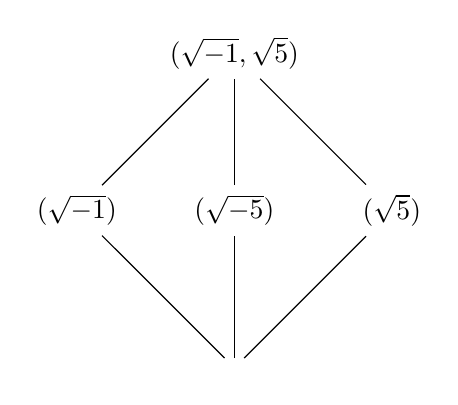
\begin{tikzpicture}
\node (Q) at (0,0) {$\Q$};
\node (Q15) at (0,4) {$\Q(\sqrt{-1}, \sqrt{5})$};
\node (Q1) at (-2,2) {$\Q(\sqrt{-1})$};
\node (Qm) at (0,2) {$\Q(\sqrt{-5})$};
\node (Q5) at (2,2) {$\Q(\sqrt{5})$};

\draw (Q)--(Q1);
\draw (Q)--(Qm);
\draw (Q)--(Q5);
\draw (Q1)--(Q15);
\draw (Qm)--(Q15);
\draw (Q5)--(Q15);
\end{tikzpicture}
\hspace{1in}
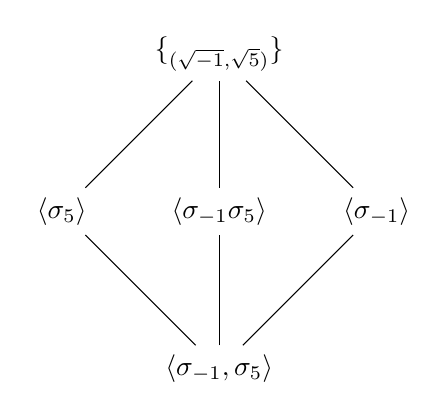
\begin{tikzpicture}
\node (Q) at (0,0) {$\langle{}\sigma_{-1}, \sigma_{5}\rangle{}$};
\node (Q15) at (0,4) {$\{\id_{\Q(\sqrt{-1}, \sqrt{5})}\}$};
\node (Q1) at (-2,2) {$\langle{}\sigma_{5}\rangle{}$};
\node (Qm) at (0,2) {$\langle{}\sigma_{-1} \sigma_{5}\rangle{}$};
\node (Q5) at (2,2) {$\langle{}\sigma_{-1}\rangle{}$};

\draw (Q)--(Q1);
\draw (Q)--(Qm);
\draw (Q)--(Q5);
\draw (Q1)--(Q15);
\draw (Qm)--(Q15);
\draw (Q5)--(Q15);
\end{tikzpicture}
\end{center}
In these two diagrams, algebraic objects in corresponding positions correspond by the galois correspondence, namely
\begin{align*}
K_{i}
&\mapsto
\Aut(K : K_{i})
\\
\fixedField(H_{i})
&\mapsfrom
H_{i}
\end{align*}
where we denote $K = \Q(\sqrt{-1}, \sqrt{5})$.

Part \ref{itm : e03q7c}: Observe that $\alpha = \sqrt{-1} + \sqrt{5} \in \Q(\sqrt{-1}, \sqrt{5})$ (because fields are closed under the field operations), so
\begin{align*}
\Q(\alpha)
\subseteq
\Q(\sqrt{-1}, \sqrt{5})
\end{align*}
For the reverse inclusion, note that
\begin{align*}
\alpha^{-1}
=
\frac{1}{\sqrt{-1} + \sqrt{5}}
=
\frac{\sqrt{-1} - \sqrt{5}}{-1 - 5}
=
-\frac{1}{6} \sqrt{-1} + \frac{1}{6} \sqrt{5}
\end{align*}
Again, fields are closed under the field operations (including taking additive and multiplicative inverses), so the field $\Q(\alpha)$ contains $\alpha^{-1}$ and hence also
\begin{align*}
\sqrt{5}
&=
\frac{1}{2} (\alpha + 6 \alpha^{-1})
&
&\text{and}
&
\sqrt{-1}
&=
\alpha - \sqrt{5}
\end{align*}
so $\Q(\sqrt{-1}, \sqrt{5}) \subseteq \Q(\alpha)$. Together, these inclusions show that $\Q(\sqrt{-1}, \sqrt{5}) = \Q(\alpha)$, as desired.

Part \ref{itm : e03q7d}: Starting with the defining equation for $\alpha$, we successively isolate radicals and take powers to get an equation involving only $\alpha$ and the desired base field $\Q$:
\begin{align*}
\alpha
&=
\sqrt{-1} + \sqrt{5}
&
&\Rightarrow
&
(\alpha - \sqrt{5})^{2}
&=
-1
&
&\Leftrightarrow
&
\alpha^{2} + 6
&=
2 \sqrt{5} \alpha
\\
&
&
&\Rightarrow
&
(\alpha^{2} + 6)^{2}
&=
20 \alpha^{2}
&
&\Leftrightarrow
&
\alpha^{4} - 8 \alpha^{2} + 36
&=
0
\end{align*}
Viewing this last equation as a polynomial evaluated at $t = \alpha$, we define
\begin{align*}
f
=
t^{4} - 8 t^{2} + 36
\end{align*}
By construction, $f(\alpha) = 0$, and by inspection, $f$ is monic. To show that $f = m_{\alpha, \Q}$, it remains only to show that $f$ is irreducible. One way to show this is to use Exercises \ref{sec : e03q6}\ref{itm : e03q7d} (which implies that $[\Q(\sqrt{-1}, \sqrt{5}) : \Q] = 4$) and \ref{sec : e03q7}\ref{itm : e03q7c} (which shows that $\Q(\alpha) = \Q(\sqrt{-1}, \sqrt{5})$):
\begin{align*}
\deg m_{\alpha, \Q}
=
[\Q(\alpha) : \Q]
=
[\Q(\sqrt{-1}, \sqrt{5}) : \Q]
=
4
\end{align*}
The fact that $f(\alpha) = 0$ implies that $m_{\alpha, \Q} \divides f$, say $f = g m_{\alpha, \Q}$. Both $m_{\alpha, \Q}$ and $f$ have degree $4$, so (using the fact that $\Q[t]$ is an integral domain, because $\Q$ is)
\begin{align*}
\deg f
&=
\deg(g m_{\alpha, \Q})
=
\deg g + \deg m_{\alpha, \Q}
&
&\Leftrightarrow
&
\deg g
&=
\deg f - \deg m_{\alpha, \Q}
=
0
\end{align*}
Thus $g \in \Q[t]$ is a nonzero constant, hence a unit. Because $m_{\alpha, \Q}$ is irreducible by definition of minimal polynomial, and $f = g m_{\alpha, \Q}$, we conclude that $f$ is irreducible.}% End solution.



\section{Exercise \ref{sec : e03q8}}
\label{sec : e03q8}

\noindent{}This exercise, combined with the theory of solvable groups, shows that the general quintic (and hence the general polynomial of degree $n \geq 5$) cannot be solved by radicals.

Let $f = t^{5} - 6 t + 3 \in \Q[t]$, and let $K_{f} \subseteq \C$ be the splitting field for $f$ in $\C$.
\begin{enumerate}[label=(\alph*)]
\item\label{itm : e03q8a} Prove that $f$ is irreducible in $\Q[t]$. Deduce that $5 \divides [K_{f} : \Q]$.
\item\label{itm : e03q8b} Prove that $f$ has exactly three zeros in $\R$ and exactly two zeros in $\C - \R$. You may use the values in the table below in your proof.
\begin{center}
\begin{tabular}{r|r r r r r}
$t$		&	$-2$		&	$-1$	&	$0$	&	$1$	&	$2$	\\
\hline
$f(t)$		&	$-17$	&	$8$	&	$3$	&	$-2$	&	$23$	\\
$f'(t)$	&	$74$		&	$-1$	&	$-6$	&	$-1$	&	$74$
\end{tabular}
\end{center}
\item\label{itm : e03q8c} Let $\tau_{\C} : \C \rightarrow \C$ denote the automorphism of $\C$ of complex conjugation (that is, for all $a, b \in \R$, $\tau_{\C}(a + b i) = a - b i$), and let $\tau \in \Aut(K_{f} : \Q)$ be the restriction of $\tau_{\C}$ to $K_{f}$. Prove that $\tau$ fixes the three real zeros of $f$ and swaps the two non-real complex ones.
\item\label{itm : e03q8d} Justify why $K_{f} : \Q$ is galois. Deduce that $\Gal(K_{f} : \Q) \isomorphism S_{5}$, the symmetric group on five elements. \fontHint{You may use without proof the fact that $S_{5}$ is generated by $\{\sigma_{2}, \sigma_{5}\}$, where $\sigma_{m} \in S_{5}$ is an $m$-cycle.}
\end{enumerate}

\spaceSolution{0in}{% Begin solution.
Part \ref{itm : e03q8a}: View $f \in \Z[t]$. Then the Eisenstein--Sch\"{o}nemann criterion with prime $p = 3$ applies to $f$: $3$ does not divide the leading coefficient, $3$ divides all other coefficients, and $3^{2}$ does not divide the constant term. Thus $f$ is irreducible in $\Z[t]$. Gau\ss{}'s lemma then implies that $f$ is irreducible in $\Q[t]$.

To show that $5 \divides [K_{f} : \Q]$, consider constructing the splitting field $K_{f}$ for $f$ in $\C$ by starting from $\Q$ and adjoining one zero of $f$ at a time. Let $\alpha_{1}, \ldots, \alpha_{5}$ be the zeros of $f$ in $\C$,% Begin footnote.
\footnote{A priori, a polynomial might have repeated zeros, but we know $f$ does not. Why?} % End footnote.
and recall that $K_{f} = \Q(\alpha_{1}, \ldots, \alpha_{5})$. Then by the tower law,% Begin footnote.
\footnote{To simplify notation, for $m \in \{0, \ldots, 5\}$, let $K_{m} = \Q(\alpha_{1}, \ldots, \alpha_{m})$, with the convention that $K_{0} = \Q$. Then for each $m \in \{1, \ldots, 5\}$, $K_{m} = K_{m - 1}(\alpha_{m})$, and equation \eqref{eq : e03q8 tower law} writes as
\begin{align*}
[K_{5} : K_{0}]
=
[K_{5} : K_{4}] \cdots [K_{1} : K_{0}]
\end{align*}%
}% End footnote.
\begin{align}
[K_{f} : \Q]
=
[\Q(\alpha_{1}, \ldots, \alpha_{5}) : \Q]
=
[\Q(\alpha_{1}, \ldots, \alpha_{4})(\alpha_{5}) : \Q(\alpha_{1}, \ldots, \alpha_{4})] \cdots [\Q(\alpha_{1}) : \Q]%
\label{eq : e03q8 tower law}
\end{align}
Because $\alpha_{1}$ is a zero of $f$ and $f$ is irreducible (in fact, $f$ is the minimal polynomial of each $\alpha_{m}$ over $\Q$), we have
\begin{align*}
[\Q(\alpha_{1}) : \Q]
=
\deg m_{\alpha_{1}, \Q}
=
\deg f
=
5
\end{align*}
Thus equation \eqref{eq : e03q8 tower law} implies that $5 \divides [K_{f} : \Q]$, as desired.

Part \ref{itm : e03q8b}: View $f \in \Q[t]$ as a function $f : \R \rightarrow \R$. Because the rule of assignment for this function is a polynomial, the function is continuous. Thus the intermediate value theorem applies: From the table of values of $f(t)$, we see that $f$ has zeros on the intervals $(-2, -1)$, $(0, 1)$, and $(1, 2)$. Thus $f$ has at least three real zeros. To show that $f$ has at most three real zeros, consider the derivative
\begin{align*}
f'
=
D_{t} f
=
5 t^{4} - 6
\end{align*}
viewed as a function $\R \rightarrow \R$. If $f$ had four real zeros, then the sign of $f'(t)$ would have to change at least four times, so by the intermediate value theorem, $f'$ would have at least three real zeros. However, $f'$ has precisely two real zeros, both of multiplicity one. By the fundamental theorem of algebra, $f$ has $\deg f = 5$ zeros in $\C$, and we have shown that exactly three of them are real, so we conclude that $f$ has exactly two zeros in $\C \setminus \R$.

Alternatively, one can use Descartes's rule of signs: Let $g \in \R[t]$, say $g = a_{n} t^{n} + \ldots + a_{0}$, with $a_{n} \neq 0$. (For simplicity, omit terms with a zero coefficient.) Then the number of positive real zeros of $g$, counted with multiplicity, equals the number of sign changes of the coefficients of $g(t)$, minus $2 k$ for some $k \in \integersNonnegative$. As a corollary, the number of negative real zeros of $g$, counted with multiplicity, equals the number of sign changes of the coefficients of $g(-t)$, minus $2 k$ for some $k \in \integersNonnegative$. Applying this to $f$,
\begin{align*}
f(t)
&=
t^{5} - 6 t + 3
&
f(-t)
&=
-t^{5} + 6 t + 3
\end{align*}
we get that $f$ has either $0$ or $2$ positive real zeros, and exactly $1$ negative real zero. Because $f(0) = 3 \neq 0$, it follows that $f$ has exactly $1$ or $3$ real zeros. The table of values of $f(t)$ and the intermediate value theorem allow us to distinguish these cases and conclude that exactly $3$ real zeros. It follows that the other two zeros of $f$ in $\C$ guaranteed by the fundamental theorem of algebra must be nonreal.

Part \ref{itm : e03q8c}: Because the coefficients of $f$ are in $\Q \subseteq \R$, any complex zeros of $f$ must come in complex conjugate pairs. We have shown that $f$ has exactly two nonreal complex zeros, so they must be complex conjugates, and are therefore swapped by $\tau$. Because $\tau_{\C}$ fixes $\R$, it follows that $\tau$ fixes the real zeros of $f$.

Part \ref{itm : e03q8d}: $K_{f}$ is a splitting field for $f \in \Q[t]$, and $f$ is separable,% Begin footnote.
\footnote{We can prove that $f$ is separable in various ways:
\begin{enumerate}
\item Our analysis of the zeros of $f$ proves it from the definition: In part \ref{itm : e03q8b} we showed that $f$ has three distinct real zeros, and our work in parts \ref{itm : e03q8b} and \ref{itm : e03q8c} showed that $f$ has two distinct nonreal complex zeros. Thus all the zeros of $f$ are distinct.
\item Alternatively, by part \ref{itm : e03q8a}, $f \in \Q[t]$ is irreducible; and the field of coefficients, $\Q$, is perfect (implied by $\characteristic \Q = 0$). Therefore $f$ is separable.
\end{enumerate}} % End footnote.
so $K_{f} : \Q$ is galois. Hence% Begin footnote.
\footnote{The first equality uses the fact that $K_{f} : \Q$ is galois. The inequality uses the theory of splitting fields: Think of the ``worst-case'' scenario when constructing a splitting field of $f$ by adjoining one zero at a time. Another way to see the inequality is to argue directly on $\Gal(K_{f} : \Q)$: An automorphism in the galois group must send a zero of a polynomial to another (possibly the same) zero of that polynomial. That is, automorphisms in the galois group permute the zeros of a polynomial defined over the base field. Moreover, an automorphism in the galois group is completely determined by its action on the generators of the extension field; here, $K_{f} = \Q(\alpha_{1}, \ldots, \alpha_{5})$, where $\{\alpha_{1}, \ldots, \alpha_{5}\}$ is the set of (five) distinct zeros of $f$ in $K_{f}$. From this, we conclude that $\Gal(K_{f} : \Q)$ is a subgroup of $\symmetricGroup_{5}$.}% End footnote.
\begin{align*}
\order \Gal(K_{f} : \Q)
=
[K_{f} : \Q]
\leq
(\deg f)!
=
5!
\end{align*}
In part \ref{itm : e03q8a} we showed that $5 \divides [K_{f} : \Q]$. It follows that $\order \Gal(K_{f} : \Q) = 5 q$, where $q \in \Z$ is not divisible by $5$. By the Sylow theorems, $\Gal(K_{f} : \Q)$ contains a Sylow $5$-subgroup, which must contain an element of order $5$. The only elements in $\symmetricGroup_{5}$ of order $5$ are $5$-cycles, so $\Gal(K_{f} : \Q)$ contains a $5$-cycle. In part \ref{itm : e03q8c} we showed that $\tau \in \Gal(K_{f} : \Q)$ swaps the two nonreal complex zeros and fixes the other zeros of $f$, so $\tau$ is a $2$-cycle. We now appeal to the conveniently provided fact that a subgroup of $\symmetricGroup_{5}$ that contains a $2$-cycle and a $5$-cycle is necessarily the whole group $\symmetricGroup_{5}$ to conclude that $\Gal(K_{f} : \Q) \isomorphism \symmetricGroup_{5}$.}% End solution.